\documentclass{article} % For LaTeX2e
\usepackage{nips2015style/nips15submit_e,times}

% Set the typeface to Times Roman
\usepackage{amsmath, amssymb}
\usepackage{graphicx}
\usepackage{algpseudocode}
\usepackage{hyperref}
\usepackage{natbib}
\usepackage{color}
\usepackage{algorithm}
\usepackage{subcaption}

\definecolor{mydarkblue}{rgb}{0,0.08,0.45}
\hypersetup{ %
    pdftitle={},
    pdfauthor={},
    pdfsubject={},
    pdfkeywords={},
    pdfborder=0 0 0,
    pdfpagemode=UseNone,
    colorlinks=true,
    linkcolor=mydarkblue,
    citecolor=mydarkblue,
    filecolor=mydarkblue,
    urlcolor=mydarkblue,
    pdfview=FitH}

% Math typesetting.
\newcommand{\vx}{\mathbf{x}}
\newcommand{\vX}{\mathbf{X}}
\newcommand{\vw}{\mathbf{w}}
\newcommand{\vv}{\mathbf{v}}
\newcommand{\vr}{\mathbf{r}}
\newcommand{\vg}{\mathbf{g}}
\newcommand{\vI}{\mathbf{I}}
\newcommand{\vzero}{\bf{0}}
\newcommand{\ones}[1]{\mat{1}_{#1}}
\newcommand{\eye}[1]{\mat{E}_{#1}}
\newcommand{\tra}{^{\mathsf{T}}}
\newcommand{\vect}[1]{{\bf{#1}}}
\newcommand{\mat}[1]{\mathbf{#1}}
\newcommand{\pderiv}[2]{\frac{\partial #1}{\partial #2}}
\newcommand{\npderiv}[2]{\nicefrac{\partial #1}{\partial #2}}
\newcommand{\argmin}{\operatornamewithlimits{argmin}}
\newcommand{\argmax}{\operatornamewithlimits{argmax}}
\newcommand{\expect}{\mathbb{E}}
\newcommand{\expectargs}[2]{\mathbb{E}_{#1} \left[ {#2} \right]}
\newcommand{\var}{\mathbb{V}}
\newcommand{\varL}{\mathcal{L}}
\def\iid{i.i.d.\ }
\def\simiid{\overset{\mbox{\tiny iid}}{\sim}}
\newcommand{\defeq}{\mathrel{:\mkern-0.25mu=}}
\newcommand{\Normal}{\mathcal{N}}
\newcommand{\Nt}[3]{\mathcal{N}\!\left(#1 \middle| #2,#3\right)}
\newcommand{\N}[2]{\mathcal{N}\!\left(#1,#2\right)}
\DeclareMathOperator{\KLop}{KL}
\newcommand{\KL}[2]{\KLop \left(#1 \middle \| #2 \right)}

% Symbol definitions.
\newcommand{\distinit}{q_0(\params, \vv)}
\newcommand{\data}{\vx}

%% \newcommand{\params}{\vx}
\newcommand{\params}{\mathbf{\theta}}
\newcommand{\trans}{T}
\newcommand{\paramsrv}{\vX}  % Random variable.
\newcommand{\numsteps}{T}
\newcommand{\decay}{\gamma}
\newcommand{\decays}{{\boldsymbol{\decay}}}
\newcommand{\stepsize}{\alpha}
\newcommand{\stepsizes}{{\boldsymbol{\stepsize}}}
\newcommand{\gradparams}{\nabla L(\params_t, t)}
\DeclareMathOperator{\SGD}{SGD}
\newcommand{\entropy}{S}
\newcommand{\pun}{{\tilde p}}
\newcommand{\jointdist}{p(\params , \data)}
\newcommand{\posterior}{p(\params | \data)}
\newcommand{\subjointdist}[2]{p_{#1}(\params_{#2} , \data)}
\newcommand{\subjointdistminibatch}[1]{\tilde{p}(\params_{#1} , \data)}
\newcommand{\reals}{\mathbb{R}}
\newcommand{\bigo}[1]{\mathcal{O}\left(#1\right)}
\newcommand{\trace}[1]{\text{Tr}\left[#1\right]}
\newcommand{\loss}{L(\params)}

\makeatletter
\renewcommand*{\@fnsymbol}[1]{\ensuremath{\ifcase#1\or \dagger\or \ddagger\or
   \mathsection\or \mathparagraph\or \|\or **\or \dagger\dagger
   \or \ddagger\ddagger \else\@ctrerr\fi}}
\makeatother


\title{Early Stopping as \\ Nonparametric Variational Inference}

\author{
David Duvenaud \thanks{ \hspace{1em}Equal contributors.} \\
\texttt{dduvenaud@seas.harvard.edu} \\
Harvard University
\And
Dougal Maclaurin $^\dagger$ \\
\texttt{dmaclaurin@seas.harvard.edu} \\
Harvard University
\And
Ryan P. Adams \\
\texttt{rpa@seas.harvard.edu} \\
Harvard University
}

\begin{document}


\maketitle

\begin{abstract}
We show that unconverged stochastic gradient descent 
can be interpreted as a procedure that samples from a nonparametric approximate posterior distribution.
This distribution is implicitly defined by the transformation of an initial distribution by a sequence of optimization steps. 
By tracking the change in entropy over these distributions during optimization, we form a scalable, unbiased estimate of a variational lower bound on the log marginal likelihood.
This bound can be used to optimize hyperparameters instead of cross-validation.
This Bayesian interpretation of SGD suggests improved, overfitting-resistant optimization procedures, and gives a theoretical foundation for early stopping and ensembling.
We investigate the properties of this marginal likelihood estimator on neural network models.
\end{abstract}

\section{Introduction}



We propose an interpretation of incomplete optimization in terms of variational Bayesian inference, and provide a simple method for estimating the marginal likelihood of the approximate posterior.
Our starting point is a Bayesian posterior distribution for a potentially complicated model, in which there is an empirical loss that can be interpreted as a negative log likelihood and regularizers that have interpretations as priors.
One might proceed with MAP inference, and perform an optimization to find the best parameters.
The main idea of this paper is that such an optimization procedure, initialized according to some distribution that can be chosen freely, generates a sequence of distributions that are implicitly defined by the action of the optimization update rule on the previous distribution.
We can treat these distributions as  approximations to the true posterior distribution.
A single optimization run for $N$ iterations represents a draw from the $N$th such distribution in the sequence.
Figure \ref{fig:cartoon} shows contours of these approximate distributions on an example posterior.
% of inferring the parameters of a univariate Guassian.

With this interpretation, the number of optimization iterations can be seen as a variational parameter, one that trades off fitting the data well against maintaining a broad (high entropy) distribution.
Early stopping amounts to optimizing the variational lower bound (or an approximation based on a validation set) with respect to this variational parameter.
%Similarly, since each optimization trajectory from a random initialization represents a sample from the variational distribution, 
Ensembling different random restarts can be viewed as taking independent samples from the variational posterior.


\subsection{Contributions}
\begin{itemize}
\item We introduce a new interpretation of optimization algorithms as samplers from a variational distribution that adapts to the true posterior, eventually collapsing around its modes.
%We also Since these variational distributions eventually collapse around local modes, 
% albeit one that does not converge to an optimal approximation.
\item We provide a scalable estimator for the entropy of these implicit distributions, allowing us to estimate a lower bound on the marginal likelihood of any model whose posterior is twice-differentiable, even on problems with millions of parameters and data points.
%Our marginal likelihood estimate provides a principled stopping criterion that depends only on the training set, and works for any twice-differentiable probabilistic model.
\item We investigate the performance of these estimators empirically on neural network models, and show that they have reasonable properties.
\end{itemize}
%Because the implicit distributions eventually collapse around local modes, early stopping can be seen as choosing a distribution with moderate amounts of entropy to prevent overfitting.

\section{Incomplete optimization as variational inference}
\label{sec:techintro}


\newcommand{\dist}[1]{\includegraphics[width=4.5cm]{../experiments/2015_03_02_funnel/6-nicer/figures/dists_#1.pdf}}%
\begin{figure*}[t]
\setlength{\tabcolsep}{1pt}
\begin{tabular}{ccc}
Initial distribution & After 150 steps & After 300 steps \\
 &  of gradient descent &  of gradient descent \\
\dist{0} &
\dist{3} &
\dist{6}
\end{tabular}
\caption{A series of distributions (blue) implicitly defined by gradient descent on an objective  (black).
%  The initial distribution from which parameters are drawn (red) doesn't match the posterior (black).
These distributions are defined by mapping each point in the initial distribution through a fixed number of iterations of optimization.
These distributions have nonparametric shapes, and eventually concentrate around the optima of the objective.}
\label{fig:cartoon}
\end{figure*}

Variational inference aims to approximate an intractable posterior distribution, $\posterior$, with another more tractable distribution, $q(\params)$.
%Ideally, the distribution~$q(\params)$ would belong to a simpler and tractable class, such as factored distributions or a parametric family.
The usual measure of the quality of the approximation is the Kullback-Leibler (KL) divergence from $q(\params)$ to $\jointdist$.
This measure provides a lower bound on the marginal likelihood of the original model;
applying Bayes' rule to the definition of $\KL{q(\params)}{\posterior}$ gives the familiar inequality:
%
\begin{align}
\log p(\data)
& \geq - \underbrace{\expectargs{q(\params)}{ -\log \jointdist }}_{\textnormal{\normalsize Energy $E[q]$}}
         \underbrace{- \expectargs{q(\params)}{\log  q(\params)}}_{\textnormal{\normalsize Entropy $S[q]$}} := \varL[q] \label{eq:varbound}
\end{align}
%
%Maximizing $\varL[q]$, the variational lower bound on the marginal likelihood, with respect to $q$ minimizes $\KL{q(\params)}{\posterior}$, the KL divergence from $q$ to the true posterior, giving the closest approximation available within the variational family.
%A convenient side effect is that we also get a lower bound on $p(\data)$, which can be used for model selection.

To perform variational inference, we require a family of distributions over which to maximize $\varL[q]$. 
Consider a general procedure to minimize the energy~$(-\log\jointdist)$ with respect to~${\params \in \reals^D}$.
The parameters~$\params$ are initialized according to some distribution~$q_0(\params)$ and updated at each iteration according to a transition operation~${\trans : \reals^D \rightarrow \reals^D}$:
%
\begin{align}
\params_0 &\sim q_0(\params) \\
\params_{t + 1} &= \trans(\params_t)
\end{align}
%
Our variational family consists of the sequence of distributions~$q_0, q_1, q_2, \ldots$,
where~$q_t(\params)$ is the distribution over~$\params_t$ generated by the above procedure.
These distributions don't have a closed form, but we can exactly sample from $q_t$ by simply running the optimizer for $t$ steps starting from a random initialization.

We cannot evaluate $\varL[q_t]$ exactly, but we can obtain an unbiased estimator.
Sampling~$\params_0$ from~$q_0$ and then applying the transition operator~$t$ times produces an exact sample~$\params_0$ from~$q_t$, by definition.
Since $\params_t$ is an exact sample from $q_t(\theta)$, $\log\subjointdist{}{t}$ is an unbiased estimator of the energy term of (\ref{eq:varbound}).
The entropy term is trickier, since we do not have access to the density $q(\params)$ directly.
However, if we know the entropy of the initial distribution, $S[q_0(\params)]$, then we can estimate $S[q_t(\params)]$ by tracking the change in entropy at each iteration, calculated by the change of variables formula. % for a probability density function.

To compute how the volume shrinks or expands due to an iteration of the optimizer, we require access to the Jacobian of the optimizer's transition operator, $J(\params)$:
%
\begin{align}
S[q_{t+1}] - S[q_t] =
  \expect_{q_t(\params_t)} \big[ \log
    \left| J(\params_t) \right| \big] \,.
\end{align}
%
Note that this analysis assumes that the mapping $T$ is bijective.
Combining these terms, we have an unbiased estimator of $\varL$ at iteration $T$,
based on the sequence of parameters, $\params_0, \ldots, \params_T$, from a single training run:
%
\begin{align}
\varL[q_T] \approx
  \underbrace{\log \subjointdist{}{T}}_{\textnormal{\normalsize Energy}} +
  \underbrace{\sum_{t=0}^{T-1} \log \left| J(\params_t) \right| + S[q_0]}_{\textnormal{\normalsize Entropy}} \,.
\label{eq:entropy-bound}
\end{align}

\paragraph{The entropy of stochastic gradient descent}
%In this section, we give an unbiased estimate for the change in entropy caused by SGD updates.
%We'll start with a na\"ive method, then in section \ref{sec:scalable-estimator}, we give an approximation that scales linearly with the number of parameters in the model.

Stochastic gradient descent is a popular optimization procedure with the following update rule:
%
\begin{align}
\params_{t+1} &=
  \params_t - \stepsize \nabla \loss,
\end{align}
%
where the $\loss$ the objective loss (or an unbiased estimator of it e.g. using minibatches)
for example ~$-\log\jointdist$, and $\stepsize$ is a `step size' hyperparameter.
Taking the Jacobian of this update rule gives the following unbiased estimator
for the change in entropy at each iteration:
%
\begin{align}
S[q_{t+1}] - S[q_t] \approx \log \left| I - \stepsize H_t(\params_t)
\right| \label{eq:exact hessian}
\end{align}
%
where $H_t$ is the Hessian of $-\log\subjointdist{t}{}$ with respect to~$\params$.


\paragraph{Estimating the Jacobian in high dimensions}
\label{sec:scalable-estimator}
The expression for the change in entropy given by (\ref{eq:exact hessian}) is impractical for large-scale problems since it requires an~$\bigo{D^3}$ determinant computation.
Fortunately, we can make a good approximation using just two Hessian-vector products, which can usually be performed in~$\bigo{D}$ time using reverse-mode differentiation \citep{pearlmutter1994fast}.
%
The idea is that since~$\stepsize\lambda_{\text{max}}$ is small, the Jacobian is just a small perturbation to the identity, and we can approximate its determinant using traces as follows:
%
\begin{align}
\log \left| I - \stepsize H \right|
& =    \sum_{i=0}^D \log\left(1 - \stepsize\lambda_i\right) 
& \geq \sum_{i=0}^D \left[- \stepsize\lambda_i 
                        - (\stepsize\lambda_i)^2 \right] \label{eq:logbound} 
& = - \stepsize \trace{H} - \stepsize^2 \trace{HH}\,.
\end{align}
%
The bound in (\ref{eq:logbound}) is just a second order Taylor expansion of~$\log(1 - x)$ about~${x = 0}$ and is valid if ${\stepsize\lambda_i < 0.68}$.
However, gradient descent is unstable anyway if ${\stepsize\lambda_{\text{max}} > 2}$, where~$\lambda_{\text{max}}$ is the largest eigenvalue of~$H_t$.
So choosing a conservative learning rate keeps this bound in the correct direction.
For sufficiently small learning rates, this bound becomes tight.

% \todo{little o terms here for clarity?}
%\todo{Mention closeness of bound.}
The trace of the Hessian can be estimated using inner products of random vectors
\citep{bai1996some}:
%
\begin{align}
\trace{H} = \expectargs{}{\vr^TH\vr}, \qquad \vr \sim \N{0}{I}\,.
\label{eq:approx-log-det}
\end{align}
%


\paragraph{Initialization objective functions}
\label{sec:priors}
What initial parameter distribution should we use for SGD?
The marginal likelihood estimate given by \eqref{eq:entropy-bound} is valid no matter which initial distribution we choose.
We use the prior as the initial distribution and log-likelihood as the objective in our experiments.


\section{Experiments}
\label{sec:experiments}

Here, we demonstrate that our marginal likelihood estimator has reasonable properties on two tasks.
Code for all experiments is available at \url{github.com/HIPS/maxwells-daemon}.

%\subsection{Boston housing data}
\paragraph{Choosing the number of training iterations}
We performed regression on the Boston housing dataset 
%[citation needed]
using a neural network with one hidden layer having 100 hidden units, sigmoidal activation functions, and no regularization.
Figure \ref{fig:housing} shows that marginal likelihood peaks at a similar place to the peak of held-out log-likelihood, which is where early stopping would occur when using a large validation set.


\begin{figure*}
\centering
\begin{minipage}{.47\textwidth}
  \centering
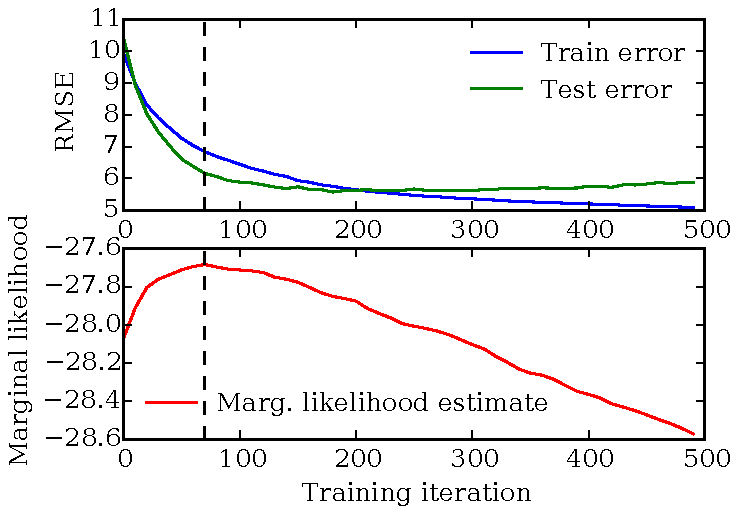
\includegraphics[width=\columnwidth]{../experiments/2015_03_01_housing/2/marglik.pdf}
\vskip -0.1in
\captionof{figure}{\emph{Top}: Training and test-set error on the Boston housing dataset.
\emph{Bottom}: Stochastic gradient descent marginal likelihood estimates.
The dashed line indicates the iteration with highest marginal likelihood.
The marginal likelihood, estimated online using only the training set, and the
test error peak at a similar number of iterations.}
\label{fig:housing}
\end{minipage}%
\hspace{1em}%
\begin{minipage}{.47\textwidth}
  \centering
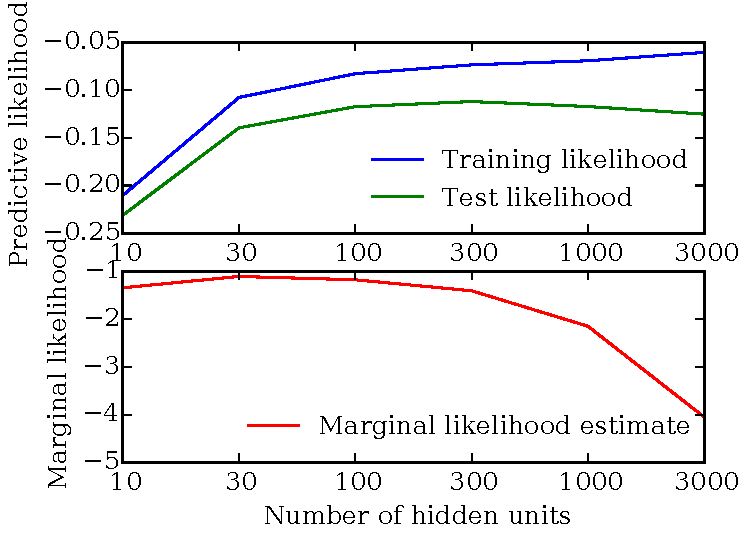
\includegraphics[width=\columnwidth]{../experiments/2015_03_03_vary_width/7_hidden_units_higher_learnrate/vary_widths.pdf}
\vskip -0.1in
\captionof{figure}{\emph{Top}: Training and test-set likelihood as a function of the number of hidden units in the first layer of a neural network.
\emph{Bottom}: Stochastic gradient descent marginal likelihood estimates.
In this case, the marginal likelihood over-penalizes high numbers of hidden units. 
}
\label{fig:num hiddens}
\end{minipage}
\end{figure*}


\paragraph{Choosing the number of hidden units}
Figure \ref{fig:num hiddens} shows marginal likelihood estimates as a function of the number of hidden units in the hidden layer of a neural network trained on 50,000 MNIST handwritten digits.
The largest network trained in this experiment contains 2 million parameters.

\section{Limitations}
\label{sec:limitations}
Using only a single sample to estimate both the expected likelihood as well as the entropy of an entire distribution will necessarily have high variance under some circumstances.
These problems could conceivably be addressed by ensembling, which has an interpretation as taking multiple exact independent samples from the implicit posterior.

Second, as parameters converge, their entropy estimate (and true entropy) will continue to decrease indefinitely, making the marginal likelihood arbitrarily small.
However, in practice there is usually a limit to the degree of overfitting possible, making our marginal likelihood estimate a poor guide to generalization performance.

Finally, figure \ref{fig:cartoon} shows that the distribution implied by SGD collapses to a small portion of the true posterior early on, and continues to shrink as optimization proceeds.
However, the point of early stopping is not that the intermediate distributions are particularly good approximations, but simply that they are better than the point masses that occur when optimization has converged.

%Estimating marginal likelihood is known to be sharp-P hard in general.
%When do we expect the estimate of the marginal likelihood to be poor?

\section{Related work}

Our method can be seen as a special case of \citet{Bridging14}, who showed that any set of stochastic dynamics, even those not satisfying detailed balance, can be used to implicitly define a variational distribution.
%
\citet{hardt2015train} give theoretical results showing that the smaller the number of training epochs, the better the generalization performance of models trained using SGD.
\citet{Dustin15} examine the properties of SGD as an estimator, and show that a variant that averages parameter updates has improved statistical efficiency.

One possible method to deal with over-zealous reduction in entropy by SGD would be to add noise to the dynamics.
In the case of Gaussian noise, we would recover Langevin dynamics~\citep{neal2011mcmc}.


%Optimization algorithms with random initializations implicitly define a series of distributions which converge to posterior modes.
%We showed that these nonparametric distributions can be seen as variational approximations to the true posterior. %when the optimization objective is a log-likelihood.

%, and allows the optimization of hyperparameters without a validation set.

%\subsection{Acknowledgements}
%We are grateful to Roger Grosse, Miguel Hern\'andez-Lobato, Matthew Johnson, and Oren Rippel for helpful discussions.
%We thank Analog Devices International and Samsung Advanced Institute of Technology for their support.

\bibliography{references.bib}
\bibliographystyle{uai2015stylefiles/icml2015}

\end{document}
